\documentclass[12pt, a4paper]{report}
\usepackage{style}


\title{Foundation Of Operations Research \\ \textit{Exercises}}
\author{Christian Rossi}
\date{Academic Year 2023-2024}

\begin{document}

\maketitle

\newpage

\begin{abstract}
    Operations Research is the branch of applied mathematics dealing with quantitative methods to analyze and solve
    complex real-world decision-making problems. 
    
    The course covers some fundamental concepts and methods of Operations Research pertaining to graph optimization, 
    linear programming and integer linear programming. 
    
    The emphasis is on optimization models and efficient algorithms with a wide range of important applications in 
    engineering and management.  
\end{abstract}

\newpage

\tableofcontents

\newpage

\chapter{Exercise session I}
    \section{Linear programming modeling}
        A bank has a capital of $C$ billions of Euro and two available stocks:
        \begin{enumerate}
            \item With an annual revenue of $15\%$ and risk factor of $\dfrac{1}{3}$. 
            \item With an annual revenue of $25\%$ and risk factor of $1$.
        \end{enumerate}
        The risk factor represents the maximum fraction of the stock value that can be lost. A risk factor of $25\%$ implies that, if stocks are bought for $100$ euro up to $25$ euro 
        can be lost. It is required that at least half of $C$ is risk-free. The amount of money used to buy stocks of two must not be larger than two times that used to buy stocks of one. 
        At least $\dfrac{1}{6}$ of C must be invested into one. 
        
        Give a Linear Programming formulation for the problem of determining an optimal portfolio for which the profit is maximized. 
        Solve the problem graphically.
    \subsection*{Solution}
        \begin{itemize}
            \item The parameters are: 
                \begin{itemize}
                    \item The quantity of available capital $C$. 
                \end{itemize}
            \item The decision variables are:
                \begin{itemize}
                    \item The amount of money invested in stock of type one $x_1$. 
                    \item The amount of money invested in stock of type two $x_2$. 
                \end{itemize}
            \item The objective function is: 
                \[\max{\left[0.15x_1+0.25x_2\right]}\]
            \item The constraints are:
                \begin{itemize}
                    \item Maximum capital: 
                        \[x_1+x_2 \leq C\]
                    \item Half of the invested capital is risk-free:
                        \[\dfrac{1}{3}x_1+x_2 \leq \dfrac{C}{2}\]
                    \item The amount of money used to buy stocks of two must not be larger than two times that used to buy stocks of one:
                        \[x_2 \leq 2x_1\]
                    \item At least $\dfrac{1}{6}$ of $C$ must be invested into one: 
                        \[x_1 \geq \dfrac{1}{6}C\]
                    \item Constraint on the variables:
                        \[x_1,x_2 \geq 0\]
                \end{itemize}
        \end{itemize}
        To solve the problem graphically, we must identify the feasible region in $\mathbb{R}^2$ that satisfies the constraints. To draw a constraint, it suffices to find any two points 
        that satisfy it with equality (as an equation). The border of the constraint is then represented by the only line containing such points. There are two possible ways to identify 
        which of the two half planes is the feasible one:
        \begin{itemize}
            \item In the first one, it suffices to pick a random point and checking whether it satisfies the constraint. If it does, the half space to which the point belongs is the
            feasible one, otherwise the other half space is.
            \item Alternatively, we can consider the gradient of the constraint and compare it to the direction of the inequality. 
        \end{itemize}
        The region found with the constraints is the following:
        \begin{figure}[H]
            \centering
            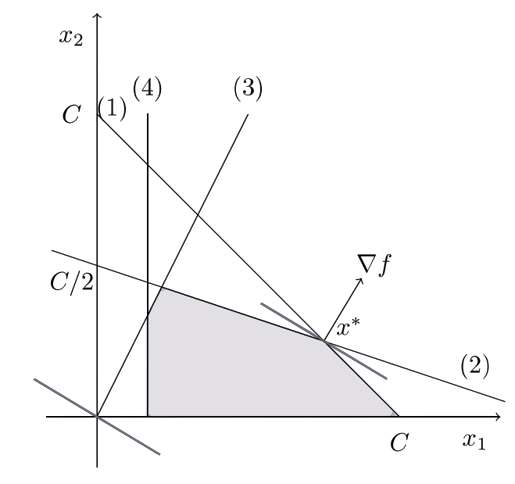
\includegraphics[width=0.3\linewidth]{images/plane.png}
        \end{figure}
        The feasible region is as shown in the picture. To find the feasible point where the objective function attains its maximal value, we can draw the level curves 
        $f(x_1,x_2)=0.15x_1+0.25x_2=z$ where each level curve is the set of points whose objective function value is equal to $z$, for any constant $z$. 
        
        Since $f$ is linear, the level curve $f(x_1,x_2) = z$ is a line, orthogonal to its gradient, and parametric in $z$. When $z$ is increased, we obtain parallel level lines that 
        move towards the direction of the gradient $\nabla f (x_1,x_2)$. 

        Note that, by starting with $z = 0$ and by increasing it in a continuous way, the level lines of f will first intersect the feasible region at $\left(\dfrac{C}{6}, 0\right)$, and then, 
        increasing $z$, at any other point, until the intersection is empty. The last feasible point having a nonempty intersection is the maximizer of $f$ over the feasible set. 
        In this problem there is a single maximizer. The maximizer, denoted by $x^{*}$, can be found as the solution to the following linear system: 
        \[
        \begin{cases}
            x_1+x_2 = C \\
            \dfrac{1}{3}x_1+x_2 = \dfrac{C}{2}
        \end{cases} 
        \]
        which yields $x^{*}=\left( \dfrac{3C}{4},\dfrac{C}{4} \right)$, where $f(x^{*})=\dfrac{7C}{40}$.

    \newpage

    \section{Linear programming modeling}
        A refinery produces two types of gasoline, mixing three basic oils according to the following gasoline mixture rules:
        \begin{table}[H]
            \centering
            \begin{tabular}{c|ccc|c|}
            \cline{2-5}
            \textbf{}                        & \textbf{Oil 1} & \textbf{Oil 2} & \textbf{Oil 3} & \textbf{Revenue} \\ \hline
            \multicolumn{1}{|c|}{Gasoline A} & $\leq 30\%$    & $\geq 40\%$    & -              & 5.5              \\
            \multicolumn{1}{|c|}{Gasoline B} & $\leq 40\%$    & $\geq 10\%$    & -              & 4.5              \\ \hline
            \end{tabular}
        \end{table}
        The last column of the previous table indicates the profit (euro/barrel). The availability of each type of oil (in barrel) and the cost (euro/barrel) are as follows:
        \begin{table}[H]
            \centering
            \begin{tabular}{c|c|c}
            \textbf{Oil} & \textbf{Availability} & \textbf{Cost} \\ \hline
            1            & 3 000                 & 3             \\
            2            & 2 000                 & 6             \\
            3            & 4 000                 & 4            
            \end{tabular}
        \end{table}
        Give a Linear Programming formulation for the problem of determining a mixture that maximizes the profit (difference between revenues and costs).
    \subsection*{Solution}
        \begin{itemize}
            \item The decision variables are:
                \begin{itemize}
                    \item The amount of the $i$-th oil used to produce the $j$-th gasoline, $i \in \{1,2,3\}$ and $j \in \{A,B\}$ $x_{ij}$. 
                    \item The amount of gasoline of type $j$-th that is produced, $j \in \{A,B\}$ $y_j$. 
                \end{itemize}
            \item The objective function is: 
                \[\max{5.5y_A+4.5y_B+3(x_{1A}+x_{1B})-6(x_{2A}+x_{2B})-4(x_{3A}+x_{3B})}\]
            \item The constraints are:
                \begin{itemize}
                    \item Availability of 1: 
                        \[x_{1A}+x_{1B} \leq 3 000\]
                    \item Availability of 2:
                        \[x_{2A}+x_{2B} \leq 2 000\]
                    \item Availability of 3:  
                        \[x_{3A}+x_{3B} \leq 4 000\]
                    \item Conservation of A:
                        \[y_A=x_{1A}+x_{2A}+x_{3A}\]
                    \item Conservation of B:
                        \[y_B=x_{1B}+x_{2B}+x_{3B}\]
                    \item Minimum quantity of $A$: 
                        \[x_{1A} \leq 0.3y_A\]
                    \item Minimum quantity of $B$: 
                        \[x_{1B} \leq 0.5y_B\]
                    \item Maximum quantity of $A$: 
                        \[x_{2A} \geq 0.4y_A\]
                    \item Maximum quantity of $B$: 
                        \[x_{2B} \geq 0.1y_B\]
                    \item The variable must be non-negative: 
                        \[x_{1A},x_{2A},x_{3A},x_{1B},x_{2B},x_{3B},y_A,y_B \geq 0\]  
                \end{itemize}
        \end{itemize}

\newpage

\chapter{Exercise session II}
    \section{Linear programming modeling}
        Assume that $n$ packets of data must be routed from node $s$ to node $t$, along one of two available links, with capacity (bandwidth) $k_1=1$ Mbps and $k_2=2$ Mbps. 
        \begin{figure}[H]
            \centering
            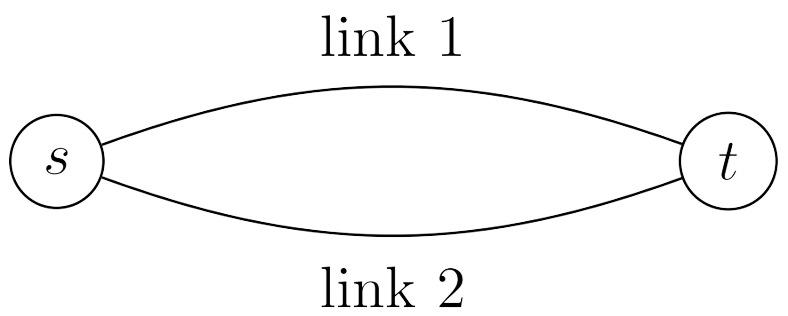
\includegraphics[width=0.4\linewidth]{images/link.png}
        \end{figure}
        The cost per unit of capacity of link $2$ is $30\%$ larger than that of link $1$. The following table indicates the quantity of capacity consumed by each packet 
        $i$, $i \in {l,\dots,n}$, and the cost to route it on link $1$. 
        \begin{table}[H]
            \centering
            \begin{tabular}{c|cc}
            \textbf{Packet} & \textbf{Consumed capacity} & \textbf{Cost on link one} \\ \hline
            1               & 0.3                        & 200                       \\
            2               & 0.2                        & 200                       \\
            3               & 0.4                        & 250                       \\
            4               & 0.1                        & 150                       \\
            5               & 0.2                        & 200                       \\
            6               & 0.2                        & 200                       \\
            7               & 0.5                        & 700                       \\
            8               & 0.1                        & 150                       \\
            9               & 0.1                        & 150                       \\
            10              & 0.6                        & 900                      
            \end{tabular}
        \end{table}
        Give an integer linear programming formulation for the problem of minimizing the total cost of routing all the packets. Give also an integer linear programming formulation for 
        the more general case where $m$ links are available. 
    \subsection*{Solution}
        The 2-link case can be formulated as the following integer linear program. 
        \begin{itemize}
            \item The sets are: 
                \begin{itemize}
                    \item The set of packets $I=\{1,\dots,n\}$. 
                    \item The set of links $J=\{1,\dots,m\}$. 
                \end{itemize}
            \item The parameters are: 
                \begin{itemize}
                    \item The capacity consumed by packet $i$, for $i \in I$ $a_i$.
                    \item The routing cost for packet $i$ on link $j$, for $i \in I,j \in J$ $c_{ij}$.
                    \item The capacity for link $j$ and $j \in J$ $k_{j}$. 
                \end{itemize}
            \item The decision variables are:
                \begin{itemize}
                    \item $x_ij$: $1$ if packet $i$ is routed on link $j$, or 0 otherwise, for $i \in I,j \in J$
                \end{itemize}
            \item The objective function is: 
                \[\min{\sum_{i \in I}{c_{ij}x_{ij}}}\]
            \item The constraints are:
                \begin{itemize}
                    \item The assignment: 
                        \[\sum_{j \in J}x_{ij} = 1\]
                    \item The capacity: 
                        \[\sum_{j \in J}a_ix_{ij} \leq k_j\]
                    \item The variables must be binary: 
                        \[x_{ij} \in \{0,1\} \:\:\:\:\:\: i \in I,j \in J\]
                \end{itemize}
        \end{itemize}
        The $m$-link formulation requires a new set of binary variables, one for each packet and link. The packet-to-link assignment is also to be explicitly introduced. 

    \newpage 

    \section{Linear programming modeling}
        A company $A$, which produces one type of high-precision measuring instrument, has to plan the production for the next 3 months. Each month, $A$ can produce at most 110 units, 
        at a unit cost of 300 Euro. Moreover, each month, up to 60 additional units produced by another company B can be bought at a unit cost of 330 Euro. Unsold units can be 
        stored. The inventory cost is of 10 Euro per unit of product, per month. Sales forecasts indicate a demand of 100, 130, and 150 units of product for the next 3 months.
        \begin{enumerate}
            \item Give a linear programming formulation for the problem of determining a production plan (direct or indirect) which minimizes the total costs, while satisfying 
                the monthly demands.
            \item Give a mixed integer linear programming formulation for the variant of the problem where production lots have a minimum size. In particular, if any strictly 
                positive quantity is produced in a given month, this quantity cannot be smaller than 15 units. 
        \end{enumerate}
    \subsection*{Solution}
        \begin{enumerate}
            \item \begin{itemize}
                    \item The sets are: 
                        \begin{itemize}
                            \item The set of months $T=\{1,2,3\}$. 
                        \end{itemize}
                    \item The parameters are: 
                        \begin{itemize}
                            \item The production capacity of $A$ $b$. 
                            \item The production capacity of $B$ $b^{'}$. 
                            \item The unit production cost for $A$ $c$. 
                            \item The unit production cost for $B$ $c^{'}$. 
                            \item The inventory cost per unit and month $m$. 
                            \item The sales forecast for month $t$, for $t \in T$ $d_t$. 
                        \end{itemize}
                    \item The decision variables are:
                        \begin{itemize}
                            \item The units produced by $A$ in month $t$, $t \in T$ $x_t$. 
                            \item The units bought from $B$ in month $t$, for $t \in T$ $x_t$ $x_t^{'}$.
                            \item The units in inventory at the end of month $t$, for $t \in T \cup \{0\}$ $z_t$. 
                        \end{itemize}
                    \item The objective function is: 
                        \[\min{\sum_{t \in T}{cx_t+c^{'}x_t^{'}+mz_t}}\]
                    \item The constraints are:
                        \begin{itemize}
                            \item The capacity of $A$: 
                                \[x_t \leq b\]
                            \item The capacity of $A$: 
                                \[x_t^{'} \leq b^{'}\]
                            \item The demand: 
                                \[x_{t-1}+x_t+x_t^{'} \geq d_t\]
                            \item The inventory balance: 
                                \[x_{t-1}+x_t+x_t^{'}-d_t = z_tt\]
                            \item The starting condition: 
                                \[z_0=0\]
                            \item The non-negative variables: 
                                \[x_t,x_t^{'},z_t \geq 0\]
                            \end{itemize}
                \end{itemize}
            \item To take into account the minimum lot size, we add the binary variables $y_t$, that is $1$ if production is active at month $t$, or $0$ otherwise, for 
                $t \in T$ and the constraints: 
                \begin{itemize}
                    \item The minimum lot size: 
                        \[x_t \geq l_{y_t}\]
                    \item The activation: 
                        \[x_t \leq M_{y_t}\]
                \end{itemize}
                where $l = 15$ is the minimum lot size, and $M$ is a large enough value, such that constraint $x_t \leq M_{y_t}$ is redundant when $y_t=1$. For instance, 
                we can choose $M = 110$. Such constraints are usually called big-$M$ constraints. 
        \end{enumerate}

\newpage

\chapter{Exercise session III}
    \section{Minimum cost spanning tree}
        Find the minimum-cost spanning tree in the graph given in the figure by using Prim's algorithm, starting from the node three. 
        \begin{figure}[H]
            \centering
            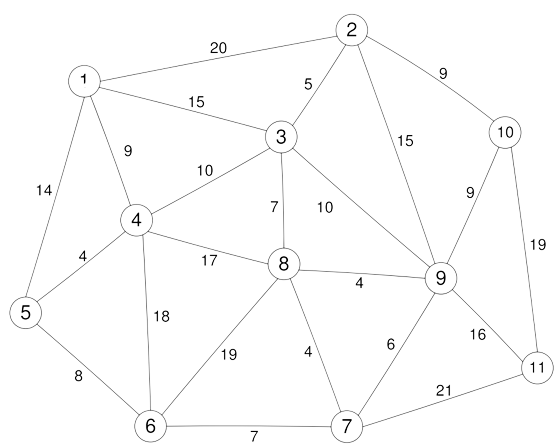
\includegraphics[width=0.4\linewidth]{images/prim.png}
        \end{figure}
    \subsection*{Solution}
    We apply Prim's algorithm, starting from node three and in the end we need to do the $10$ iterations since we have $11$ nodes. The iterations are summarized in the 
    following table: 
    \begin{table}[H]
        \centering
        \begin{tabular}{lccc}
        \hline
        \textbf{Reached nodes} & \textbf{Added edge} & \textbf{Edge cost} & \textbf{Iteration} \\ \hline
        3                      & $\{2,3\}$           & 5                  & 1                  \\
        2,3                    & $\{3,8\}$           & 7                  & 2                  \\
        2,3,8                  & $\{7,8\}$           & 4                  & 3                  \\
        2,3,7,8                & $\{8,9\}$           & 4                  & 4                  \\
        2,3,7,8,9              & $\{6,7\}$           & 7                  & 5                  \\
        2,3,6,7,8,9            & $\{5,6\}$           & 8                  & 6                  \\
        2,3,5,6,7,8,9          & $\{4,5\}$           & 4                  & 7                  \\
        2,3,4,5,6,7,8,9        & $\{2,10\}$          & 9                  & 8                  \\
        2,3,4,5,6,7,8,9,10     & $\{1,4\}$           & 9                  & 9                  \\
        1,2,3,4,5,6,7,8,9,10   & $\{9,11\}$          & 16                 & 10                 \\ \hline
        \end{tabular}
    \end{table}
    The minimum cost spanning tree that has been found has total cost $73$, and it is shown in the following figure. 
    \begin{figure}[H]
        \centering
        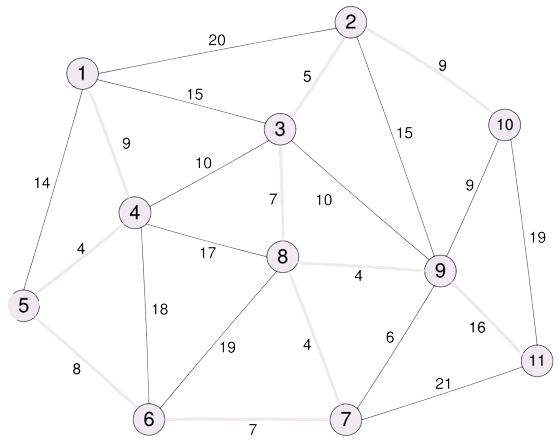
\includegraphics[width=0.4\linewidth]{images/primsol.png}
    \end{figure}

    \newpage

    \section{Kruskal's algorithm}
        In 1956 Joseph Kruskal proposed the following greedy algorithm to find a minimum cost spanning tree in an arbitrary connected undirected graph $G = (N, E)$ with a cost
        $c_e$ attached to each edge $e \in E$. 
        \begin{algorithm}[H]
            \caption{Kruskal's algorithm}
                \begin{algorithmic}[1]
                    \State sort the edges of $E$ as $\{e_1,\dots,e_m\}$ where $c_{e_1} \leq c_{e_2} \leq \dots \leq c_{e_m}$
                    \State $i \leftarrow 1$
                    \State initialize the sub graph $G' = (N, E)$ of $G$ with $F=\varnothing$
                    \While {$\left\lvert F \right\rvert < n-1$}
                        \If {the two endpoints of the edge $e_i$ belong to different connected components of the current sub graph $G^{'}$}
                            \State $F \leftarrow F \cup \{e_i\}$
                            \State merge the two connected components 
                        \EndIf 
                        \State $i \leftarrow i+1$
                    \EndWhile
                    \State \Return the spanning tree $G^{'} = (N, E)$ 
                \end{algorithmic}
        \end{algorithm}
        In other words, we order the edges by increasing (non-decreasing) cost, we consider the edges in that order and, at each step, we select the current edge (which is 
        one of the cheapest edges still available) only if it does not create a cycle with the previously selected edges. The algorithm terminates when $n-1$ edges have
        been selected. 
        \begin{enumerate}
            \item Describe an efficient way to identify/keep track of the connected components of the sub graph $G^{'}$ and to check that a new edge is creating a cycle with 
                the previously selected edges (is connecting two distinct connected components of $G^{''}$). Determine the overall computational complexity of this 
                implementation of Kruskal's algorithm. 
            \item By invoking the optimality condition for minimum-cost spanning trees, verify that Kruskal's algorithm is exact. 
            \item Find the maximum-cost spanning tree in the graph of the previous exercise by using a straightforward adaptation of Kruskal's algorithm. 
            \item Apply the Kruskal's algorithm on the graph of the previous exercise to find the minimum spanning tree. 
        \end{enumerate}
    \subsection*{Solution}
        \begin{enumerate}
            \item To identify/keep track of the connected components (subtrees) of the sub graph $G$, we use a vector $v$ with as many components as vertices in the graph, 
                where $v_i$ indicates the index of the connected component containing node $i$. At the beginning of the algorithm, we start with $v_i=i$, for $i = 1,\dots,n$. 
                When an edge $e = {i,j}$ is considered for addition to $G^{''}$, we compare the values $v_i$ and $v_j$. If $v_i \neq v_j$, then we can add the edge e to $G^{'}$ 
                because it does not create a cycle. Since the two connected components of indices $v_i$ and $v_j$ are merged, the indices are updated as follows: in the vector $v$
                we substitute each occurrence of the index of node $i$ with that of node $j$. If $v_i = v_j$, edge e is skipped because it would create a cycle. 
            \item The $m$ edges can be ordered by non-decreasing cost in $O(m\log m)$, which is $O(m \log n)$ since $m\log m \leq m\log n^2 = 2m\log n$. At most $m$ edges are 
                considered for addition to the current sub graph $G^{'}$. At each iteration, an edge $e = {i,j}$ is considered and the vector $v$ is updated (in $O(n)$) only if 
                $v_i \neq v_j$. Since a merging operation occurs exactly$ n-1$ times (a spanning tree contains $n-1$ edges), the overall complexity is $O(m\log n + m+n^2)=
                O(mlogn + n^2)$. 
            \item To verify that Kruskal's algorithm is exact, we just need to recall that the edges are considered in order of non-decreasing cost and to invoke the 
                optimality condition for minimum cost spanning tree. Since each edge e that has been discarded (not added to $F$) has a cost $c_e$ which is at least as large as 
                the cost of all the previously selected edges, it is not a cost-decreasing edge. According to the optimality condition for minimum cost spanning trees, the 
                resulting spanning tree is of minimum total cost because no cost-decreasing edge exists. 
            \item The algorithm needs $10$ iteration to find the maximum spanning tree. The iterations are summarized in the following table (remember that we order the edges,
                and we add them only if they do not create any cycle): 
                \begin{table}[H]
                    \centering
                    \begin{tabular}{lccc}
                    \hline
                    \textbf{Connected components}       & \textbf{Edge} & \textbf{Cost} & \textbf{Iteration} \\ \hline
                    $\varnothing$                       & \{7,11\}      & 21            & 1                  \\
                    \{7,11\}                            & \{1,2\}       & 20            & 2                  \\
                    \{1,2\}, \{7,11\}                   & \{6,8\}       & 19            & 3                  \\
                    \{1,2\}, \{7,11\}, \{6,8\}          & \{10,11\}     & 19            & 4                  \\
                    \{1,2\}, \{7,10,11\}, \{6,8\}       & \{4,6\}       & 18            & 5                  \\
                    \{1,2\}, \{7,10,11\}, \{4,6,8\}     & \{4,8\}       & NO            & 6                  \\
                    \{1,2\}, \{7,10,11\}, \{4,6,8\}     & \{9,11\}      & 16            & 7                  \\
                    \{1,2\}, \{7,9,10,11\}, \{46,8\}    & \{1,3\}       & 15            & 8                  \\
                    \{1,2,3\}, \{7,9,10,11\}, \{4,6,8\} & \{2,9\}       & 15            & 9                  \\
                    \{1,2,3,7,9,10,11\}, \{4,6,8\}      & \{1,5\}       & 14            & 10                 \\
                    \{1,2,3,5,7,9,10,11\}, \{4,6,8\}    & \{3,9\}       & No            & 11                 \\
                    \{1,2,3,4,5,6,7,8,9,10,11\}         & \{3,4\}       & 10            & 12                 \\ \hline
                    \end{tabular}
                \end{table}
                The spanning tree of maximum cost, of value 167, is shown in the figure. 
                \begin{figure}[H]
                    \centering
                    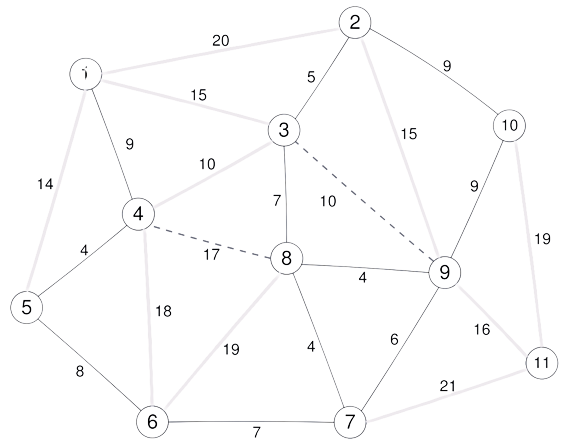
\includegraphics[width=0.4\linewidth]{images/kruskal.png}
                \end{figure}
        \end{enumerate}

    \newpage

    \section{Optimality check}
        Without applying any one of Prim's and Kruskal's algorithms, verify whether the following spanning tree is of minimum cost. 
        \begin{figure}[H]
            \centering
            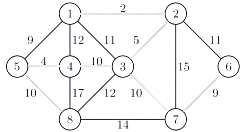
\includegraphics[width=0.5\linewidth]{images/optimality.png}
        \end{figure}
    \subsection*{Solution}
        It suffices to verify that there exists a cost decreasing edge. By inspection, we observe that, by adding edge $\{1,5\}$ to the tree, the cycle 
        $\left\langle 1,5,4,3,2,1\right\rangle$ is introduced. In such cycle, edge $\{4,3\}$ has a strictly larger cost than $\{1,5\}$. 
        \begin{figure}[H]
            \centering
            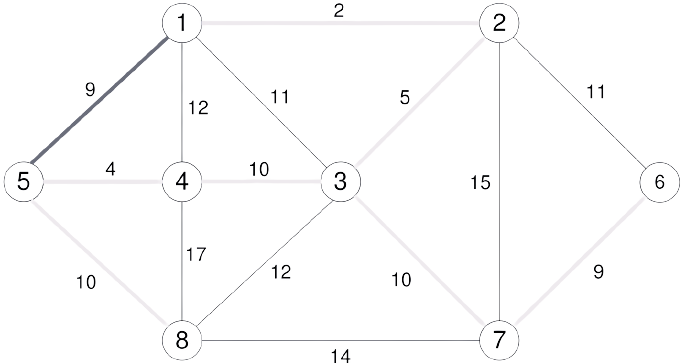
\includegraphics[width=0.5\linewidth]{images/optimality1.png}
        \end{figure}
        Therefore, by removing edge $\{4,3\}$ and adding edge $\{1,5\}$, a spanning tree of strictly smaller total cost is obtained. 
        \begin{figure}[H]
            \centering
            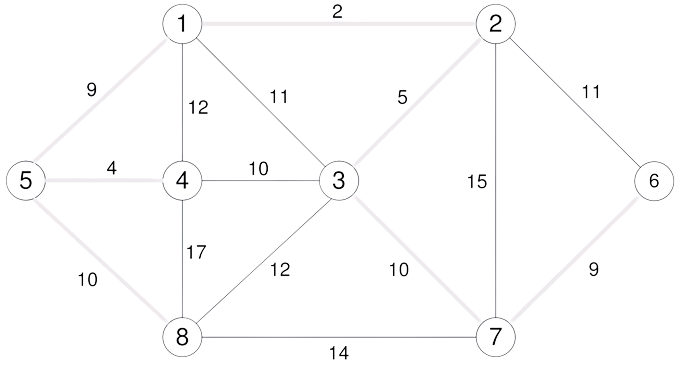
\includegraphics[width=0.5\linewidth]{images/optimality2.png}
        \end{figure}

    \newpage

    \section{Compact storage of similar sequences}
        Consider the problem of storing a large set of strings. We assume that the strings have many similar entries (they differ only in a small number of positions) and 
        we wish to store them in a compact way. This problem arises in several contexts such as when storing DNA sequences, where the characters correspond to the four DNA 
        bases. In this exercise, we consider the simplified version of the problem with only two characters. Given a set of $k$ sequences of $M$ bits, we compute for each 
        pair $i,j$, with $1 < i,j < k$, the Hamming distance between the sequences $i$ and $j$, i.e., the number of bits that need to be flipped in sequence $i$ to obtain 
        sequence $j$. This function clearly satisfies the three usual properties of a distance: non-negativity, symmetry and triangle inequality. Consider the following 
        set of $6$ sequences and the corresponding matrix $D = {d_{ij}}$ of Hamming distances: 
        \begin{enumerate}
            \item 011100011101 
            \item 101101011001 
            \item 110100111001 
            \item 101001111101 
            \item 100100111101 
            \item 010101011100 
        \end{enumerate}
        \begin{table}[H]
            \centering
            \begin{tabular}{c|cccccc}
              & 1 & 2 & 3 & 4 & 5 & 6 \\ \hline
            1 & 0 & 4 & 4 & 5 & 4 & 3 \\
            2 &   & 0 & 4 & 3 & 4 & 5 \\
            3 &   &   & 0 & 5 & 2 & 5 \\
            4 &   &   &   & 0 & 3 & 6 \\
            5 &   &   &   &   & 0 & 5 \\
            6 &   &   &   &   &   & 0
            \end{tabular}
        \end{table}
        Where, due to symmetry, only the upper triangle of the matrix is shown. In order to exploit redundancies between sequences and to save memory, we can store: one of 
        the sequences, called the reference sequence, completely and for every other sequence, only the set of bit flips that allow us to retrieve it either directly from 
        the reference sequence or from another sequence. 

        Show how the problem of deciding which differences to memorize, to minimize the total number of bits used for storage, can be reduced to the problem of finding a 
        minimum-cost spanning tree in an appropriate graph. Solve the problem for the given instance. 
    \subsection*{Solution}
        We construct a complete graph $G$ with a node for each sequence and an edge for each pair of sequences. Moreover, each edge $\{i,j\}$ is assigned a cost 
        $d_{ij}\log_2(M)$, which corresponds to the number of bits needed to store the indices of the positions in which the $i$-th and $j$-th sequences differ.
        The problem is then to look for a sub graph $G^{'}$ of $G$ of minimum total cost. Since only one sequence is completely stored, $G^{'}$ must be connected to be 
        able to retrieve any sequence. Since a sub graph of minimal cost is sought, $G^{'}$ will be acyclic. Therefore, a minimum cost spanning tree in $G$ provides an 
        optimal solution to the problem under consideration. The following minimum cost spanning tree has been found using Prim's algorithm. 
        \begin{figure}[H]
            \centering
            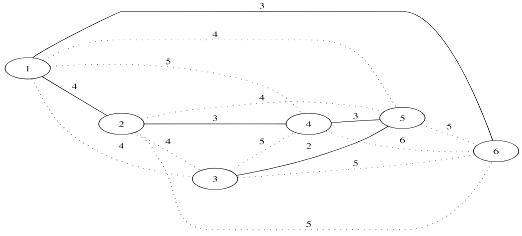
\includegraphics[width=0.8\linewidth]{images/DNA1.png}
        \end{figure}

\newpage

\chapter{Exercise session IV}
    \section{Shortest paths with non-negative costs}
        Given the following directed graph, find a set of the shortest paths from node 0 to all the other nodes, using Dijkstra's algorithm. Can we solve the problem with Dynamic 
        Programming? If yes, do so.
        \begin{figure}[H]
            \centering
            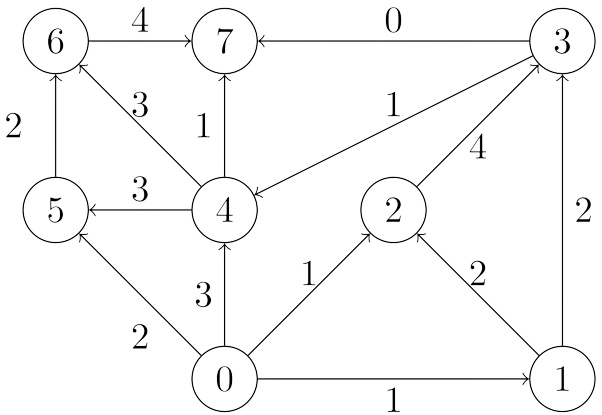
\includegraphics[width=0.35\linewidth]{images/dijk.png}
        \end{figure}
    \subsection*{Solution}
        Dijkstra's algorithm determines a set of shortest paths from a given node s to all the other nodes in the graph. It can be applied to any (directed) graph with 
        non-negative arc costs. The iteration is summarized in the following table. 
        \begin{table}[H]
            \centering
            \resizebox{\textwidth}{!}{%
            \begin{tabular}{|c|cc|cc|cc|cc|cc|cc|cc|cc|cc|}
            \hline
            \multicolumn{1}{|l|}{Iteration} & \multicolumn{1}{l}{0} & \multicolumn{1}{l|}{} & \multicolumn{1}{l}{1} & \multicolumn{1}{l|}{} & \multicolumn{1}{l}{2} & \multicolumn{1}{l|}{} & \multicolumn{1}{l}{3} & \multicolumn{1}{l|}{} & \multicolumn{1}{l}{4} & \multicolumn{1}{l|}{} & \multicolumn{1}{l}{5} & \multicolumn{1}{l|}{} & \multicolumn{1}{l}{6} & \multicolumn{1}{l|}{} & \multicolumn{1}{l}{7} & \multicolumn{1}{l|}{} & \multicolumn{1}{l}{8} & \multicolumn{1}{l|}{} \\ \hline
            Node                           & L                     & p                     & L                     & p                     & L                     & p                     & L                     & p                     & L                     & p                     & L                     & p                     & L                     & p                     & L                     & p                     & L                     & p                    \\
            0                              & 0                     & -                     & 0                     & -                     & 0                     & -                     & 0                     & -                     & 0                     & -                     & 0                     & -                     & 0                     & -                     & 0                     & -                     & 0                     & -                    \\
            1                              & $\infty$              & -                     & 1                     & 0                     & 1                     & 0                     & 1                     & 0                     & 1                     & 0                     & 1                     & 0                     & 1                     & 0                     & 1                     & 0                     & 1                     & 0                    \\
            2                              & $\infty$              & -                     & 1                     & 0                     & 1                     & 0                     & 1                     & 0                     & 1                     & 0                     & 1                     & 0                     & 1                     & 0                     & 1                     & 0                     & 1                     & 0                    \\
            3                              & $\infty$              & -                     & $\infty$              & -                     & 3                     & 1                     & 3                     & 1                     & 3                     & 1                     & 3                     & 1                     & 3                     & 1                     & 3                     & 1                     & 3                     & 1                    \\
            4                              & $\infty$              & -                     & 3                     & 0                     & 3                     & 0                     & 3                     & 0                     & 3                     & 0                     & 3                     & 0                     & 3                     & 0                     & 3                     & 0                     & 3                     & 0                    \\
            5                              & $\infty$              & -                     & 2                     & 0                     & 2                     & 0                     & 2                     & 0                     & 2                     & 0                     & 2                     & 0                     & 2                     & 0                     & 2                     & 0                     & 2                     & 0                    \\
            6                              & $\infty$              & -                     & $\infty$              & -                     & $\infty$              & -                     & $\infty$              & -                     & 4                     & 5                     & 4                     & 5                     & 4                     & 5                     & 4                     & 5                     & 4                     & 5                    \\
            7                              & $\infty$              & -                     & $\infty$              & -                     & $\infty$              & -                     & $\infty$              & -                     & $\infty$              & -                     & 3                     & 3                     & 3                     & 3                     & 3                     & 3                     & 3                     & 3                    \\ \hline
            \end{tabular}%
            }
        \end{table}
        Graphically, we have that the final graph is the following. 
        \begin{figure}[H]
            \centering
            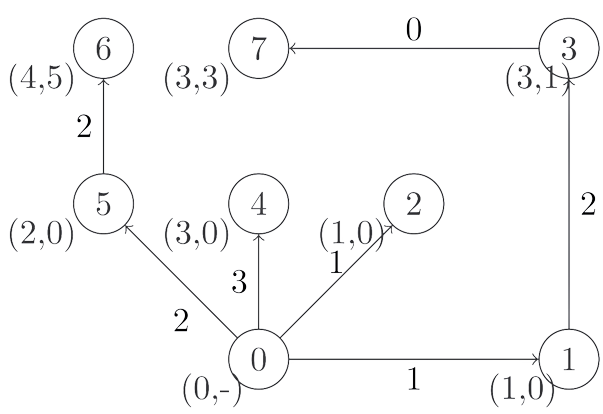
\includegraphics[width=0.5\linewidth]{images/dijksol.png}
        \end{figure}
        A topological order can be obtained as follows. At iteration $i$, for $i = 1, \dots , n$, pick a node with no incoming arcs, label it as node $i$, remove it from 
        the graph, iterate until all nodes are removed, or there is no node with no incident arcs. The graph we are dealing with is acyclic, and its node indices already 
        correspond to a topological order. The Dynamic Programming technique can therefore be applied. The steps are the following: 
        \begin{itemize}
            \item $L(0) = 0, p(0) = 0$
            \item $L(1) = L(0) + c_{01} = 1, p(1) = 0$
            \item $L(2) = \min\{L(0) + c_{02}, L(1) + c_{12}\} = \min\{0 + 1, 1 + 2\} = 1, p(2) = 0$
            \item $L(3) = \min\{L(1) + c_{13}, L(2) + c_{23}\} = \min\{1 + 2, 1 + 4\} = 3, p(3) = 1$
            \item $L(4) = \min\{L(0) + c_{04}, L(3) + c_{34}\} = \min\{0 + 3, 3 + 1\} = 3, p(4) = 0$
            \item $L(5) = \min\{L(0) + c_{05}, L(4) + c_{45}\} = \min\{0 + 2, 3 + 3\} = 3, p(5) = 0$
            \item $L(6) = \min\{L(4) + c_{46}, L(5) + c_{56}\} = \min\{3 + 3, 2 + 2\} = 3, p(6) = 5$
            \item $L(7) = \min\{L(3) + c_{37}, L(4) + c_{47}, L(6) + c_{67}\} = \min\{3 + 0, 3 + 1, 4 + 4\} = 3, p(7) = 3$
        \end{itemize}

    \newpage
    
    \section{Shortest paths with negative costs}
        Given the following directed graph, find the shortest paths between all pairs of nodes, or show that the problem is ill-posed by exhibiting a circuit of total 
        negative cost.
        \begin{figure}[H]
            \centering
            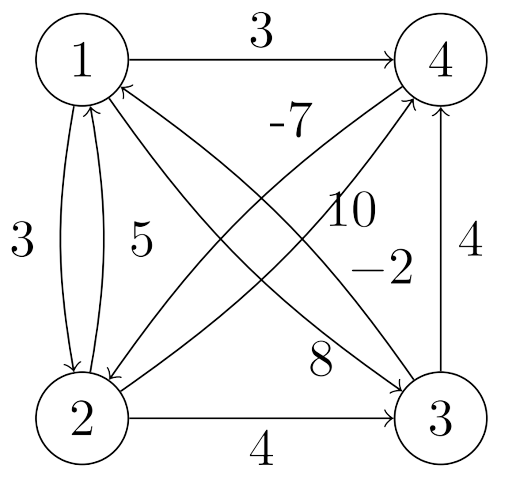
\includegraphics[width=0.3\linewidth]{images/neg.png}
        \end{figure}
    \subsection*{Solution}
        Since the graph contains negative arc costs, we use Floyd-Warshall's algorithm that finds the shortest path between each pair of nodes, or establishes that the 
        problem is ill-posed by exhibiting a circuit of negative cost. The graph can contain cycles, but such cycles must be of non-negative cost. The steps are the following: 
        \begin{enumerate}
            \item The initial configuration is the following. 
                \begin{table}[H]
                    \centering
                    \begin{tabular}{c|cccccc|cccc}
                    D & 1        & 2        & 3        & 4  & $\:\:\:\:\:\:$ & P & 1 & 2 & 3 & 4 \\ \cline{1-5} \cline{7-11} 
                    1 & 0        & 3        & 8        & 3  &                & 1 & 1 & 1 & 1 & 1 \\
                    2 & 5        & 0        & 4        & 10 &                & 2 & 2 & 2 & 2 & 2 \\
                    3 & -2       & $\infty$ & 0        & 4  &                & 3 & 3 & 3 & 3 & 3 \\
                    4 & $\infty$ & -7       & $\infty$ & 0  &                & 4 & 4 & 4 & 4 & 4
                    \end{tabular}
                \end{table}
            \item The first iteration is the following. 
                \begin{enumerate}
                    \item $d_{21} + d_{12} = 8 > d_{22} = 0$
                    \item $d_{21} + d_{13} = 13 > d_{23} = 4$
                    \item $d_{21} + d_{14} = 8 < d_{24} = 10 \Rightarrow$ update $d_{24}, p_{24}$
                    \item $d_{31} + d_{12} = 1 < d_{32} = \infty \Rightarrow$ update $d_{32}, p_{32}$
                    \item $d_{31} + d_{13} = 6 > d_{33} = 0$
                    \item $d_{31} + d_{14} = 1 < d_{34} = 4 \Rightarrow$ update $d_{34}, p_{34}$
                    \item $d_{41} + d_{ij} = \infty (\forall i, j)$
                \end{enumerate}
                The matrices become: 
                \begin{table}[H]
                    \centering
                    \begin{tabular}{c|cccccc|cccc}
                    D & 1        & 2  & 3        & 4 & $\:\:\:\:\:\:$ & P & 1 & 2 & 3 & 4 \\ \cline{1-5} \cline{7-11} 
                    1 & 0        & 3  & 8        & 3 &                & 1 & 1 & 1 & 1 & 1 \\
                    2 & 5        & 0  & 4        & 8 &                & 2 & 2 & 2 & 2 & 1 \\
                    3 & -2       & 1  & 0        & 1 &                & 3 & 3 & 1 & 3 & 1 \\
                    4 & $\infty$ & -7 & $\infty$ & 0 &                & 4 & 4 & 4 & 4 & 4
                    \end{tabular}
                \end{table}
            \item The second iteration is the following. 
                \begin{enumerate}
                    \item $d_{12} + d_{21} = 8 > d_{11} = 0$
                    \item $d_{12} + d_{23} = 7 < d_{13} = 8 \Rightarrow$ update $d_{13}, p_{13}$
                    \item $d_{12} + d_{24} = 11 > d_{24} = 3$
                    \item $d_{32} + d_{21} = 6 > d_{31} = -2$
                    \item $d_{32} + d_{23} = 5 > d_{33} = 0$
                    \item $d_{32} + d_{24} = 9 > d_{34} = 1$
                    \item $d_{42} + d_{21} = -2 < d_{41} = \infty \Rightarrow$ update $d_{41}, p_{41}$
                    \item $d_{42} + d_{23} = -3 < d_{43} = \infty \Rightarrow$ update $d_{43}, p_{43}$
                    \item $d_{42} + d_{24} = 1 > d_{44} = 0$
                \end{enumerate}
                The matrices become: 
                \begin{table}[H]
                    \centering
                    \begin{tabular}{c|cccccc|cccc}
                    D & 1  & 2  & 3  & 4 & $\:\:\:\:\:\:$ & P & 1 & 2 & 3 & 4 \\ \cline{1-5} \cline{7-11} 
                    1 & 0  & 3  & 7  & 3 &                & 1 & 1 & 1 & 2 & 1 \\
                    2 & 5  & 0  & 4  & 8 &                & 2 & 2 & 2 & 2 & 1 \\
                    3 & -2 & 1  & 0  & 1 &                & 3 & 3 & 1 & 3 & 1 \\
                    4 & -2 & -7 & -3 & 0 &                & 4 & 2 & 4 & 2 & 4
                    \end{tabular}
                \end{table}
            \item The third iteration is the following. 
                \begin{enumerate}
                    \item $d_{13} + d_{31} = 5 > d_{11} = 0$
                    \item $d_{13} + d_{32} = 8 > d_{12} = 3$
                    \item $d_{13} + d_{34} = 8 > d_{14} = 3$
                    \item $d_{23} + d_{31} = 2 < d_{21} = 5 \Rightarrow$ update $d_{21}, p_{21}$
                    \item $d_{23} + d_{32} = 5 > d_{22} = 0$
                    \item $d_{23} + d_{34} = 5 < d_{24} = 8 \Rightarrow$ update $d_{24}, p_{24}$
                    \item $d_{43} + d_{31} = -5 < d_{41} = -2 \Rightarrow$ update $d_{41}, p_{41}$
                    \item $d_{43} + d_{32} = -2 > d_{42} = -7$
                    \item $d_{43} + d_{34} = -2 < d_{44} = 0 \Rightarrow$ update $d_{44}, p_{44}$
                \end{enumerate}
                The matrices become: 
                \begin{table}[H]
                    \centering
                    \begin{tabular}{c|cccccc|cccc}
                    D & 1  & 2  & 3  & 4  & $\:\:\:\:\:\:$ & P & 1 & 2 & 3 & 4 \\ \cline{1-5} \cline{7-11} 
                    1 & 0  & 3  & 7  & 3  &                & 1 & 1 & 1 & 2 & 1 \\
                    2 & 2  & 0  & 4  & 5  &                & 2 & 3 & 2 & 2 & 1 \\
                    3 & -2 & 1  & 0  & 1  &                & 3 & 3 & 1 & 3 & 1 \\
                    4 & -5 & -7 & -3 & -2 &                & 4 & 3 & 4 & 2 & 1
                    \end{tabular}
                \end{table}
        \end{enumerate}
        We obtain $d_{44} = -2 < 0$ and the algorithm halts: we found a circuit with a total negative cost of $-2$, $\left\langle (4, 2),(2, 3),(3, 1),(1, 4) \right\rangle $.

    \newpage

    \section{Dynamic Programming}
        A company must buy a new machine and then determine a renewal (maintenance-replacement) plan for the next 5 years, making sure that, at any point in time, the available
        machine works properly. At the beginning of each year of the planning horizon, the company must decide whether to keep the old machine or to substitute it with a new 
        machine. The maintenance costs and the expected revenue (when the machine is sold) depend on how old the machine. They are indicated in the following table.
        \begin{table}[H]
            \centering
            \begin{tabular}{ccc}
            \hline
            \textbf{Years} & \textbf{Maintenance (k)} & \textbf{Revenue when sold (k)} \\ \hline
            0              & 2                        & -                              \\
            1              & 4                        & 7                              \\
            2              & 5                        & 6                              \\
            3              & 9                        & 2                              \\
            4              & 12                       & 1                              \\ \hline
            \end{tabular}
        \end{table}
        To avoid high maintenance costs of an old machine, the machine can be sold at the beginning of the second, third, fourth, and fifth year, and a new one can be bought. 
        For the sake of simplicity, we suppose that a new machine always costs 12k Euro. Show that the problem of determining a machine renewal plan of minimum total net cost 
        (total cost for buying/rebuying the machine + maintenance costs - total revenue) can be solved via Dynamic Programming by finding the shortest path in an ad hoc 
        directed acyclic graph. Find an optimal renewal plan. Is it unique?
    \subsection*{Solution}
        Consider a directed graph with six nodes: nodes 1 to 5 are associated to the beginning of each year, while node 6 corresponds to the end of the 5 years time horizon.
        For each pair $i, j$, with $i, j = 1, \dots , 5$ and $i < j$, the arc $(i, j)$ that represents the choice of buying a machine at the beginning of year $i$ and 
        selling it at the beginning of year $j$. The cost $c_{ij}$ of arc $(i, j)$ is defined as the net cost of the corresponding partial renewal plan from the beginning of 
        year $i$ to the beginning of year $j$, namely: 
        \[c_{ij}=c_b+\left( \sum_{k=0}^{j-i-1}m_k \right)-r_{j-i}\]
        where $c_b$ is the buying cost of 12000 Euro, $m_k$ is the annual maintenance cost for a machine that is $k$ years old, and $r_k$ is the selling price of a machine 
        which is $k$ years old. We obtain the following directed acyclic graph:
        \begin{figure}[H]
            \centering
            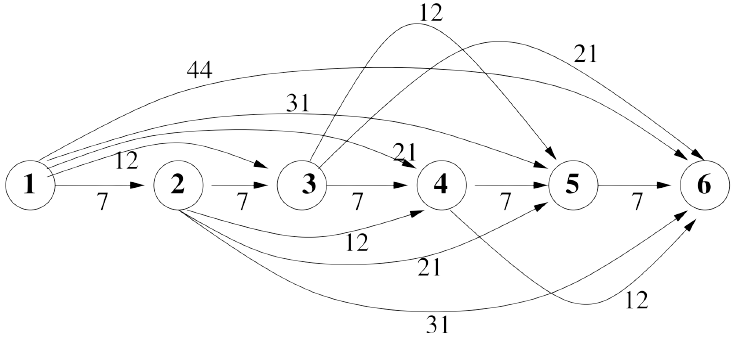
\includegraphics[width=0.75\linewidth]{images/dag.png}
        \end{figure}
        Any path from node 1 to node 6 corresponds to a (complete) renewal plan whose total net cost is equivalent to the total cost of the path. To look for the shortest 
        path from node 1 to node 6, we apply the Dynamic Programming algorithm, obtaining:
        \begin{enumerate}
            \item $L(1) = 0$
            \item $L(2) = 7, p(2) = 1$
            \item $L(3) = 12, p(3) = 1$
            \item $L(4) = 19, p(4) = 3$
            \item $L(5) = 24, p(5) = 3$
            \item $L(6) = 31, p(6) = 5$
        \end{enumerate}
        The shortest path (of cost 31) is $\left\langle (1, 3),(3, 5),(5, 6)\right\rangle $. It amounts to buy a new machine every 2 years. Note that there are two other 
        optimal solutions: path $\left\langle (1, 2),(2, 4)(4, 6)\right\rangle $ and path $\left\langle (1, 3),(3, 4),(4, 6)\right\rangle $.

    \newpage

    \section{Project planning}
        The preparation of the apple pie has long been a tradition at Rossi's family. First the weight of the ingredients has to be determined: flour, sugar, butter, eggs, 
        apples, cream. The butter must then be melted down, and added to a mixture of flour, sugar, and eggs. Apples must be added to this new mixture, once they have been 
        peeled and cut into thin slices. The mixture can then be cooked, in the already heated oven. It is advisable to whip the cream only after the apple slices have 
        been added to the mixture. Once the cake is cooked, the cream is used to garnish it. The following table reports the time needed for each activity.
        \begin{table}[H]
            \centering
            \begin{tabular}{ccc}
            \hline
            \textbf{} & \textbf{Activity}                        & \textbf{Times (minutes)} \\ \hline
            A         & Weight the ingredients                   & 5                        \\
            B         & Melt the butter                          & 3                        \\
            C         & Mix flour, eggs and sugar                & 5                        \\
            D         & Peel the apples and cut them into slices & 10                       \\
            E         & Heat the oven                            & 20                       \\
            F         & Add butter to the mixture                & 8                        \\
            G         & Add apples to the mixture                & 4                        \\
            H         & Cook the mixture in the oven             & 40                       \\
            I         & Whip the cream                           & 10                       \\
            L         & Garnish                                  & 5                        \\ \hline
            \end{tabular}
        \end{table}
        Draw the graph (with activities associated to arcs) which represents the project precedence relations. Determine the minimum total completion time of the project 
        as well as the earliest times and the latest times associated to each node. Identify the critical activities and draw Gantt's chart at earliest.
    \subsection*{Solution}
        We derive the directed graph representing the precedence relations as follows. For each activity, we introduce an arc whose cost is equivalent to the duration of the 
        activity (its two nodes represent the beginning and the end of the activity). For each precedence relation $A_i < A_j$, a fictitious arc $(i, j)$ of duration 0 is 
        introduced (dashed line) between the ending node of the arc associated to Ai and the beginning node of the arc associated to $A_j$. We include a node $s$ and, 
        for each activity without predecessors associated to arc $(v, w)$, we add the arc $(s, v)$ of cost 0. Similarly, we include a node $t$ and, for each activity 
        without successors associated to arc $(v, w)$, we add the arc $(w, t)$ of cost 0.
        \begin{figure}[H]
            \centering
            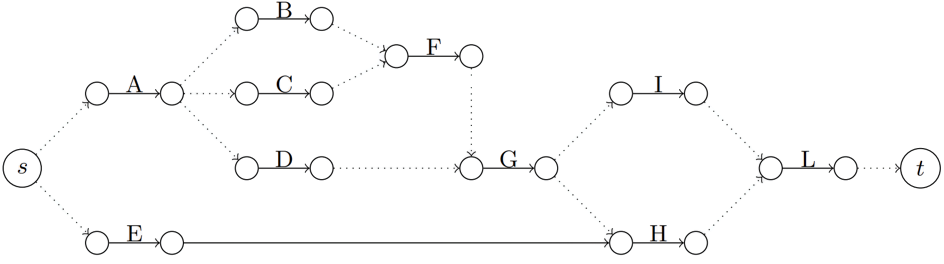
\includegraphics[width=0.9\linewidth]{images/prog.png}
        \end{figure}
        By deleting some fictitious arcs while paying attention not to create any unwanted precedence relations, we obtain the following more compact directed 
        acyclic graph representing the project. 
        \begin{figure}[H]
            \centering
            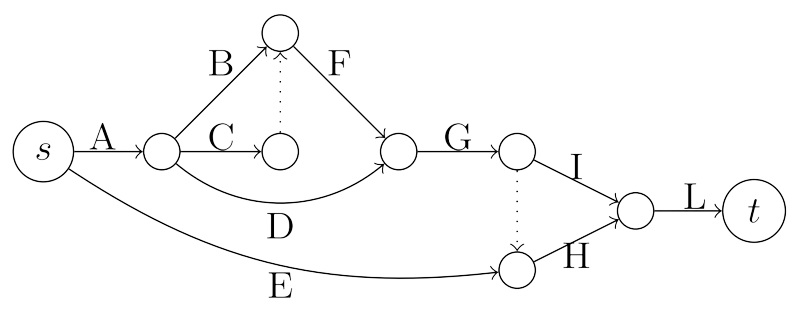
\includegraphics[width=0.75\linewidth]{images/prog1.png}
        \end{figure}
        We use the Critical Path Method to determine, for each node $v$ of the graph, the at earliest and at latest times, denoted by $T_{min_v}$ and respectively $T_{max_v}$.
        The algorithm exploits the topological order of the nodes and consists of two phases where Dynamic Programming is applied considering the n nodes in the 
        increasing/decreasing order of the indices. Here is the pseudocode of the algorithm:
        \begin{algorithm}[H]
            \caption{Critical Path Method algorithm}
                \begin{algorithmic}[1]
                    \State sort the nodes topologically
                    \State $T_{min_1} \leftarrow 0$
                    \For {$j=2,\dots,n$}
                        \State $T_{min_j} \leftarrow \max\{T_{min_i} + d_{ij} | (i, j) \in \delta^{-}(j)\}$
                    \EndFor
                    \State $T_{max_n} \leftarrow T_{min_n}$
                    \For {$i=n-1,\dots,1$}
                    \State $T_{max_i} \leftarrow \min\{T_{mmax_j} - d_{ij} | (i, j) \in \delta^{+}(i)\}$
                \EndFor
                \end{algorithmic}
        \end{algorithm}
        After ordering topologically the nodes, we obtain the following earliest times and latest times:
        \begin{figure}[H]
            \centering
            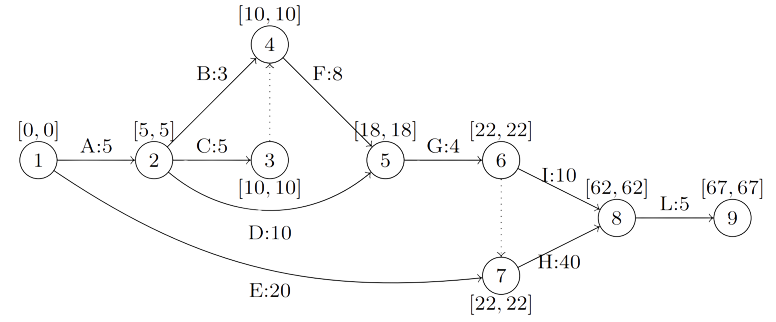
\includegraphics[width=0.9\linewidth]{images/prog2.png}
        \end{figure}
        The slacks for the activities are: 
        \begin{itemize}
            \item $\sigma(A) = T_{max_2} - T_{min_1} - d_{12} = 5 - 0 - 5 = 0$
            \item $\sigma(B) = T_{max_4} - T_{min_2} - d_{24} = 10 - 5 - 3 = 2$
            \item $\sigma(C) = T_{max_3} - T_{min_2} - d_{23} = 10 - 5 - 5 = 0$
            \item $\sigma(D) = T_{max_5} - T_{min_2} - d_{25} = 18 - 5 - 10 = 3$
            \item $\sigma(E) = T_{max_6} - T_{min_1} - d_{16} = 22 - 0 - 20 = 2$
            \item $\sigma(F) = T_{max_5} - T_{min_4} - d_{45} = 18 - 10 - 8 = 0$
            \item $\sigma(G) = T_{max_6} - T_{min_5} - d_{56} = 22 - 18 - 4 = 0$
            \item $\sigma(H) = T_{max_8} - T_{min_7} - d_{78} = 62 - 22 - 40 = 0$
            \item $\sigma(I) = T_{max_8} - T_{min_6} - d_{68} = 62 - 22 - 10 = 30$
            \item $\sigma(L) = T_{max_9} - T_{min_8} - d_{89} = 67 - 62 - 7 = 0$
        \end{itemize}
        The critical activities are A, C, F, G, H, L.

    \newpage

    \section{Shortest paths with negative costs}
        Given the following directed graph, find the shortest paths between all pairs of nodes, or show that the problem is ill-posed, by exhibiting a circuit of total 
        negative cost.
        \begin{figure}[H]
            \centering
            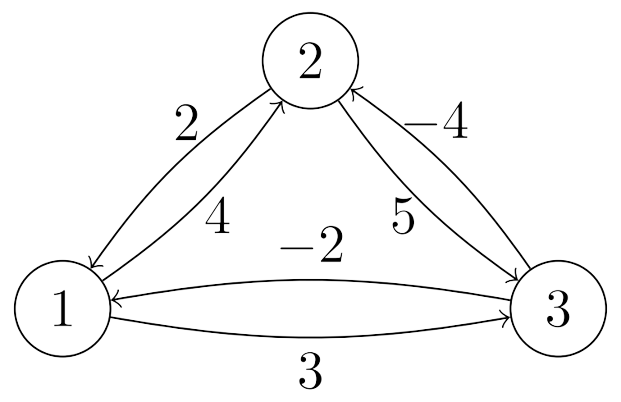
\includegraphics[width=0.3\linewidth]{images/neg1.png}
        \end{figure}
    \subsection*{Solution}
        The steps of the Warshall-Floyd's algorithm are the following:
        \begin{enumerate}
            \item The initial configuration is the following. 
                \begin{table}[H]
                    \centering
                    \begin{tabular}{c|ccccc|ccc}
                    D & 1        & 2        & 3          & $\:\:\:\:\:\:$ & P & 1 & 2 & 3  \\ \cline{1-4} \cline{6-9} 
                    1 & 0        & 4        & 3          &                & 1 & 1 & 1 & 1  \\
                    2 & 2        & 0        & 5          &                & 2 & 2 & 2 & 2  \\
                    3 & -2       & -4       & 0          &                & 3 & 3 & 3 & 3  \\ 
                    \end{tabular}
                \end{table}
            \item The first iteration is the following. 
                \begin{enumerate}
                    \item $d_{21} + d_{12} = 2 + 4 = 6 > d_{22} = 0$
                    \item $d_{21} + d_{13} = 2 + 3 = 5 = d_{23} = 5$
                    \item $d_{31} + d_{13} = -2 + 3 = 1 > d_{33} = 0$
                    \item $d_{31} + d_{12} = -2 + 4 = 2 > d_{32} = -4$
                \end{enumerate}
                The matrices become: 
                \begin{table}[H]
                    \centering
                    \begin{tabular}{c|ccccc|ccc}
                    D & 1        & 2        & 3          & $\:\:\:\:\:\:$ & P & 1 & 2 & 3  \\ \cline{1-4} \cline{6-9} 
                    1 & 0        & 4        & 3          &                & 1 & 1 & 1 & 1  \\
                    2 & 2        & 0        & 5          &                & 2 & 2 & 2 & 2  \\
                    3 & -2       & -4       & 0          &                & 3 & 3 & 3 & 3  \\ 
                    \end{tabular}
                \end{table}
            \item The second iteration is the following. 
                \begin{enumerate}
                    \item $d_{12} + d_{21} = 4 + 2 = 6 > d_{11} = 0$
                    \item $d_{12} + d_{23} = 4 + 5 = 9 > d_{13} = 3$
                    \item $d_{32} + d_{23} = -4 + 5 = 1 > d_{33} = 0$
                    \item $d_{32} + d_{21} = -4 + 2 = -2 = d_{31} = -2$
                \end{enumerate}
                The matrices become: 
                \begin{table}[H]
                    \centering
                    \begin{tabular}{c|ccccc|ccc}
                    D & 1        & 2        & 3          & $\:\:\:\:\:\:$ & P & 1 & 2 & 3  \\ \cline{1-4} \cline{6-9} 
                    1 & 0        & 4        & 3          &                & 1 & 1 & 1 & 1  \\
                    2 & 2        & 0        & 5          &                & 2 & 2 & 2 & 2  \\
                    3 & -2       & -4       & 0          &                & 3 & 3 & 3 & 3  \\ 
                    \end{tabular}
                \end{table}
            \item The third iteration is the following. 
                \begin{enumerate}
                    \item $d_{13} + d_{31} = 3 - 2 = 1 > d_{11} = 0$
                    \item $d_{13} + d_{32} = 3 - 4 = -1 < d_{12} = 4 \Rightarrow$ update $d_{12}, p_{12}$
                    \item $d_{23} + d_{32} = 5 - 4 = 1 > d_{22} = 0$
                    \item $d_{23} + d_{31} = 5 - 2 = 3 > d_{21} = 2$
                \end{enumerate}
                The matrices become: 
                \begin{table}[H]
                    \centering
                    \begin{tabular}{c|ccccc|ccc}
                    D & 1        & -1       & 3          & $\:\:\:\:\:\:$ & P & 1 & 2 & 3  \\ \cline{1-4} \cline{6-9} 
                    1 & 0        & 4        & 3          &                & 1 & 1 & 3 & 1  \\
                    2 & 2        & 0        & 5          &                & 2 & 2 & 2 & 2  \\
                    3 & -2       & -4       & 0          &                & 3 & 3 & 3 & 3  \\ 
                    \end{tabular}
                \end{table}
        \end{enumerate}

\newpage

\chapter{Exercise session V}
    \section{Maximum flow}
        Given the following network with capacities on the arcs: 
        \begin{figure}[H]
            \centering
            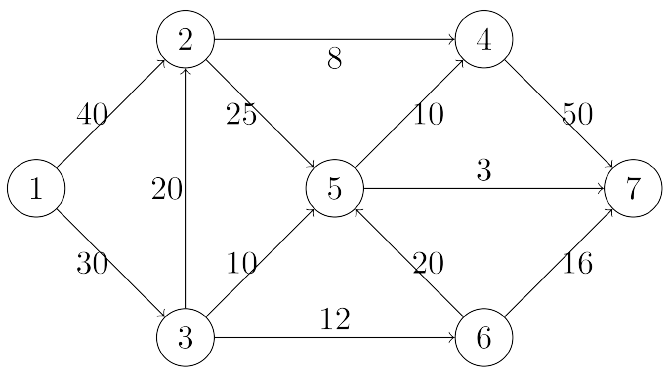
\includegraphics[width=0.5\linewidth]{images/maxfl.png}
        \end{figure}
        find a maximum flow from node $1$ to node $7$, starting from the feasible flow of value $21$ in which $x_{12} = 11$, $x_{13} = x_{36} = x_{54} = x_{65} = 10$, $x_{24} = 8$, $x_{25} = x_{57} = 3$, 
        $x_{47} = 18$, and $x_{ij} = 0$ for the remaining arcs. Determine a corresponding minimum cut.
    \subsection*{Solution}
        The initial feasible flow $\underline{x_0}$ of value $\varphi_0 = 21$ and the associated incremental (residual) network are as follows:        
        \begin{figure}[H]
            \centering
            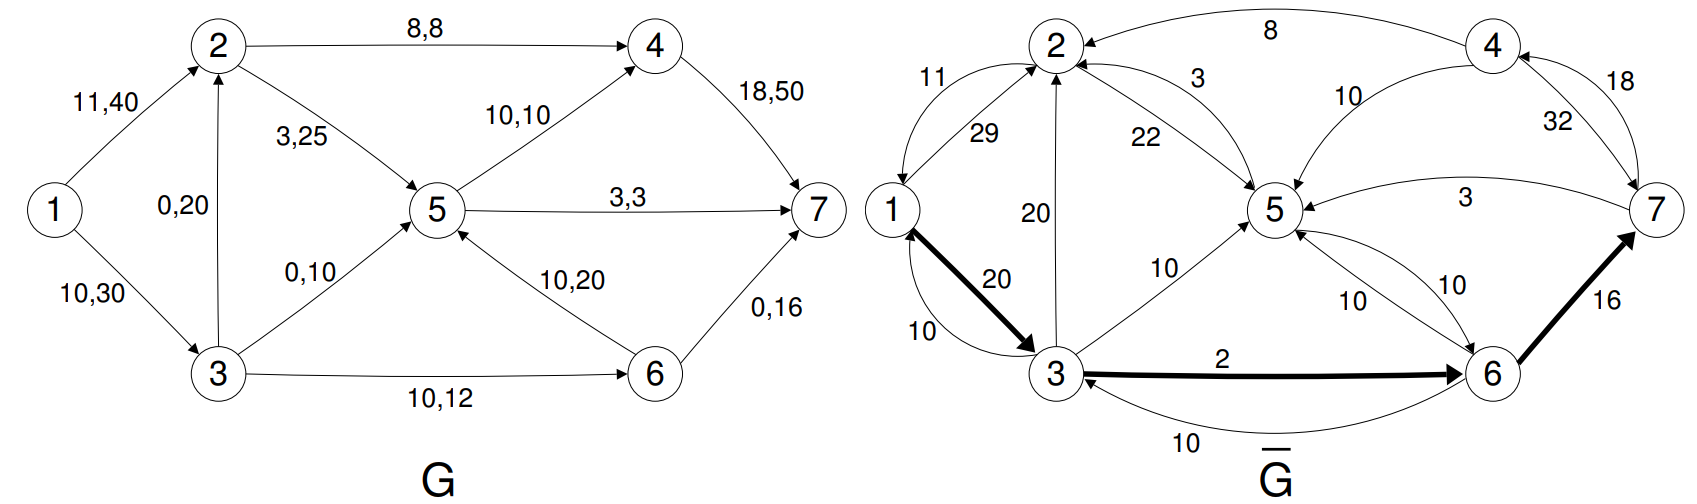
\includegraphics[width=1\linewidth]{images/flow.png}
        \end{figure}
        By sending $\delta = 2$ additional units along the path $\left\langle (1, 3),(3, 6),(6, 7)\right\rangle $, we obtain the following feasible flow 
        $x_3$ of value $\varphi_3 = 23$ and the associated residual network:
        \begin{figure}[H]
            \centering
            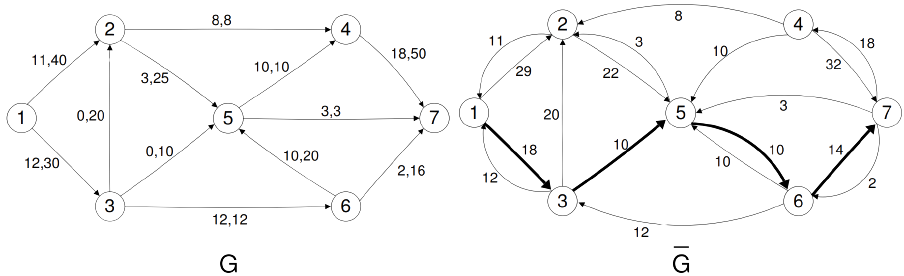
\includegraphics[width=1\linewidth]{images/flow1.png}
        \end{figure}
        Observe that all augmenting paths for this network use the backward arc $(5, 6)$. From the flow point of view, this amounts to unload arc $(6, 5)$, decreasing the amount of product flowing
        through it.

        By sending $\delta = 10$ units along the path $\left\langle (1, 3),(3, 5),(5, 6),(6, 7)\right\rangle $, we obtain the following feasible flow $x_4$ of value $\varphi_4 = 33$ 
        and the associated residual network. 
        \begin{figure}[H]
            \centering
            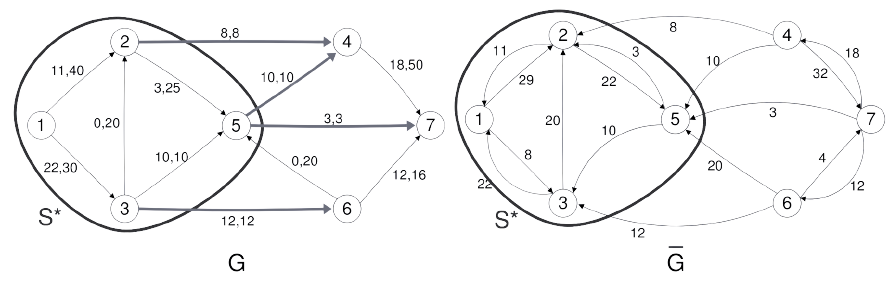
\includegraphics[width=1\linewidth]{images/flow2.png}
        \end{figure}
        No other augmenting path exists. The set $S^{*} = \{1, 2, 3, 5\}$, highlighted in blue, contains all the nodes that can be reached in $\overline{G}$ from the 
        source one. $S^{*}$ induces in the network $G$ the cut $\delta_G(S^{*})$ of minimum total capacity $k(S^{*})=33$ which is highlighted in red. Note that, 
        according to strong duality, the value $\varphi_4 = 9$ of the feasible flow $x_4$ is equal to the total capacity $k(S^{*})$ of by the cut 
        $\delta_G(S^{*}) = \{(2, 4),(3, 6),(5, 4),(5, 7)\}$ induced by $S^{*}$.
        
    \newpage 

    \section{Maximum flow and minimum cut}
        Given the following network with capacities on the arcs: 
        \begin{figure}[H]
            \centering
            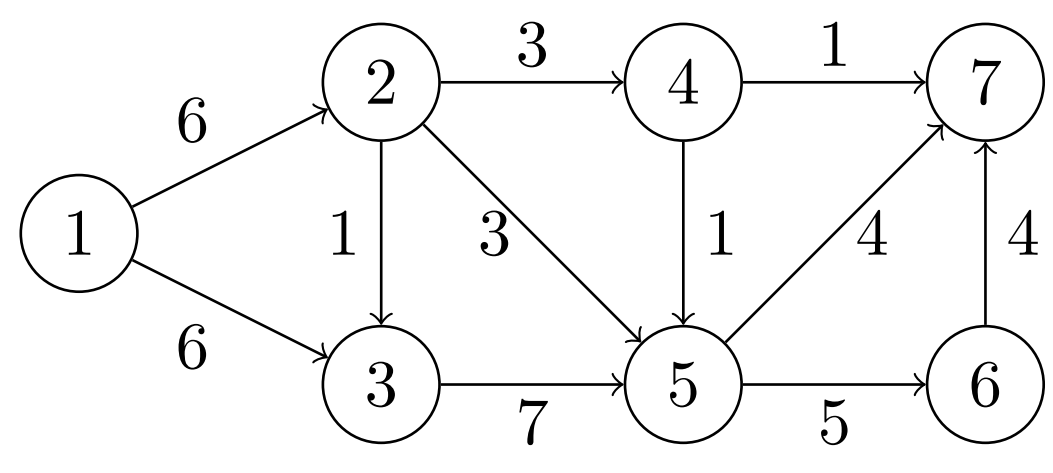
\includegraphics[width=0.5\linewidth]{images/maxcut.png}
        \end{figure}
        find a maximum (feasible) flow from node 1 to node 7, and determine a corresponding minimum (capacity) cut.
    \subsection*{Solution}
        We apply Ford-Fulkerson's algorithm. In the following figures, on the left we report the current feasible flow in the network $G$ (with on each arc the quantity 
        of product $x_{ij}$ flowing through it and its capacity $k_{ij}$) and on the right the incremental (residual) network $\overline{G}$ associated to the current 
        feasible flow.

        We start from the null feasible flow $\underline{x}_0=0$ of value $\varphi_0 = 0$. Since all arcs are empty, $\overline{G}$ is equivalent to $G$.
        \begin{figure}[H]
            \centering
            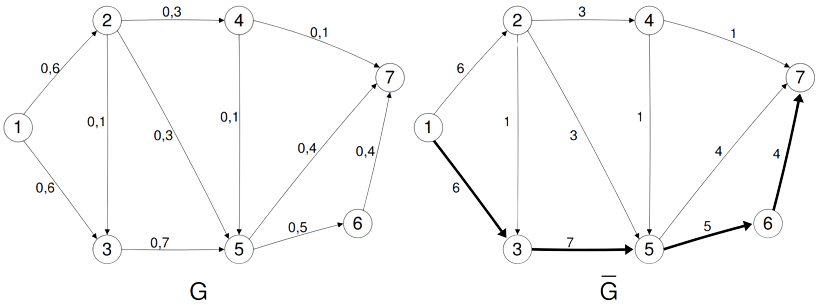
\includegraphics[width=0.9\linewidth]{images/maxcut1.png}
        \end{figure}
        Along the augmenting path $\left\langle (1, 3),(3, 5),(5, 6),(6, 7)\right\rangle $ we can send up to $\delta = 4$ additional units of product. $\delta$ is given 
        by arc $(6, 7)$ which has the smallest capacity $k_{ij}$ of all arcs on the path. Adding these $\delta=4$ units of product to the feasible flow $\underline{x}_0$, 
        we obtain the following feasible flow $\underline{x}_1$ (on the left) of value $\varphi_1 = 0 + 4 = 4$. The associated incremental (residual) network is reported 
        on the right.
        \begin{figure}[H]
            \centering
            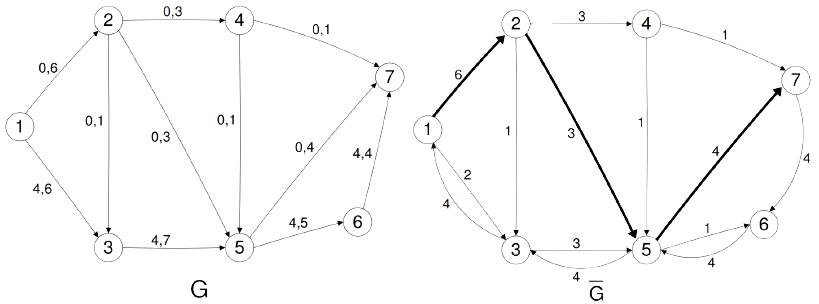
\includegraphics[width=0.9\linewidth]{images/maxcut2.png}
        \end{figure}
        Along the augmenting path $\left\langle (1, 2),(2, 5),(5, 7)\right\rangle $ we can send up to $\delta = 3$ additional units of product. $\delta$ is given by arc 
        $(2, 5)$ which has the smallest residual capacity $\underline{k}_{ij}$ of all arcs on the path. Adding these $\delta = 3$ units of product to the feasible flow 
        $\underline{x}_1$, we obtain the following feasible $\underline{x}_2$ of value $\varphi_2 = 4 + 3 = 7$. The associated incremental (residual) network is reported 
        on the right.
        \begin{figure}[H]
            \centering
            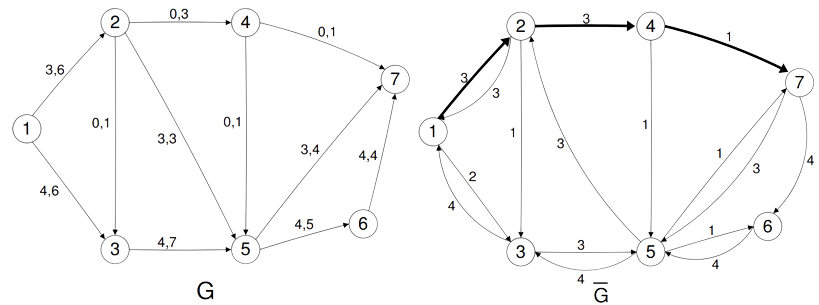
\includegraphics[width=0.9\linewidth]{images/maxcut3.png}
        \end{figure}
        Along the augmenting path $\left\langle (1, 2),(2, 4),(4, 7) \right\rangle $ we can send up to $\delta = 1$ additional units of product, where $\delta$ is given 
        by arc $(4, 7)$. We obtain the following feasible flow $\underline{x}_3$ (on the left) of value $\varphi_3 = 7 + 1 = 8$. The associated incremental (residual) 
        network is reported on the right.
        \begin{figure}[H]
            \centering
            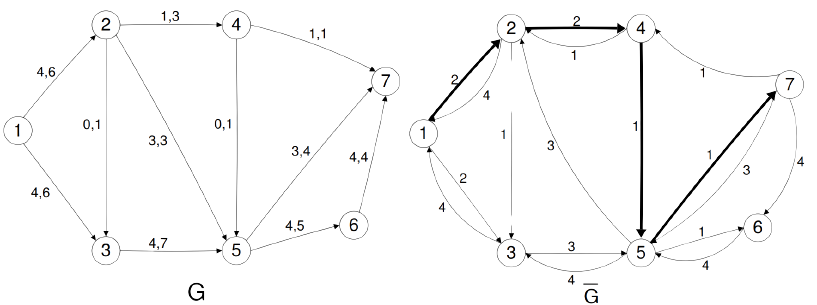
\includegraphics[width=0.9\linewidth]{images/maxcut4.png}
        \end{figure}
        Along the augmenting path $\left\langle (1, 2),(2, 4),(4, 5),(5, 7) \right\rangle $ we can send up to $\delta = 1$ additional units of product, where $\delta$ is 
        given by arc $(4, 5)$ (or $(5, 7)$). We obtain the following feasible flow $\underline{x}_4$ (on the left) of value $\varphi_4 = 8 + 1 = 9$. The associated 
        incremental (residual) network is reported on the right.
        \begin{figure}[H]
            \centering
            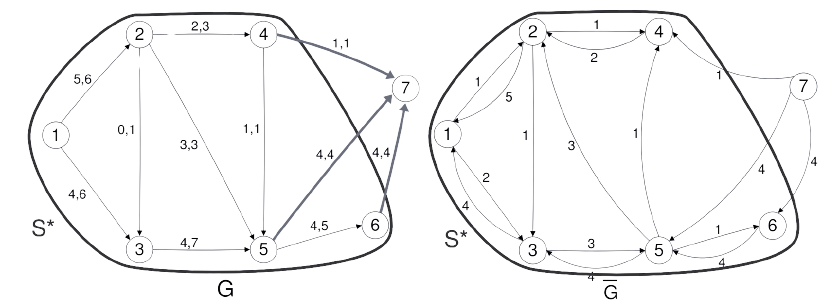
\includegraphics[width=0.9\linewidth]{images/maxcut5.png}
        \end{figure}
        Since no other augmenting path exists (no path from node 1 to node 7 in the incremental/residual network $\overline{G}$), the algorithm halts. The set 
        $S^{*} = \{1, 2, 3, 4, 5, 6\}$, highlighted in blue, contains all the nodes that can be reached from the source 1 in $\overline{G}$. $S^{*}$ induces the 
        cut $\delta(S^{*})$ of minimum total capacity $k(S^{*}) = 9$ which is highlighted in red. Note that, according to strong duality, the value $\varphi_4=9$ of the 
        feasible flow $\underline{x}_4$ is equal to the total capacity $k(S^{*})$ of the cut $\delta(S^{*}) = \{(4, 7),(5, 7),(6, 7)\}$ induced by $S^{*}$.

    \newpage

    \section{Maximum flow with node capacities}
        In maximum flow problems, how can we deal with capacities on both nodes and arcs? Find a maximum flow from node 1 to node 7 in the network of the previous exercise, 
        with a node capacity of 2 on node 6.
    \subsection*{Solution}
        The capacities on nodes can be easily reduced to capacities on arcs. Indeed, each node $i$ with a capacity $c_i$ can be substituted with two auxiliary nodes, 
        which are connected with an arc whose capacity is equal to $c_i$ and where all entering arcs entering the left node and all exiting arcs exit from the right node.
        \begin{figure}[H]
            \centering
            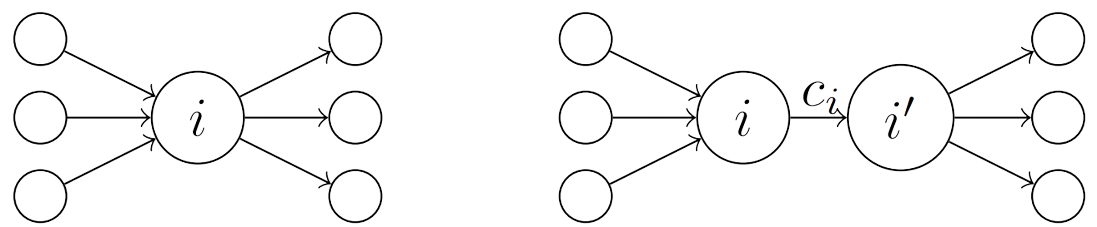
\includegraphics[width=0.5\linewidth]{images/max.png}
        \end{figure}
        The network is modified as follows. 
        \begin{figure}[H]
            \centering
            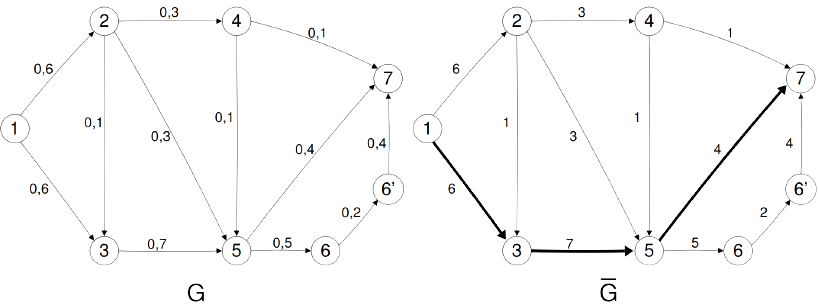
\includegraphics[width=0.9\linewidth]{images/max1.png}
        \end{figure}
        We send $\delta=4$ additional units along the path \[\left\langle (1, 3),(3, 5),(5, 7) \right\rangle\]
        \begin{figure}[H]
            \centering
            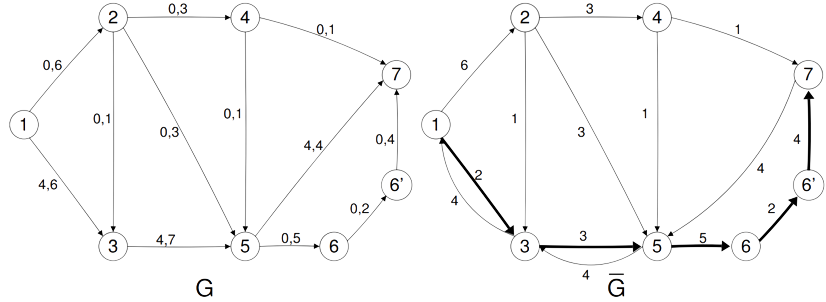
\includegraphics[width=0.9\linewidth]{images/max2.png}
        \end{figure}
        We send $\delta = 2$ additional units along the augmenting path \[\left\langle (1, 3),(3, 5),(5, 6),(6, 6^{'}),(6^{'}, 7)\right\rangle\]
        \begin{figure}[H]
            \centering
            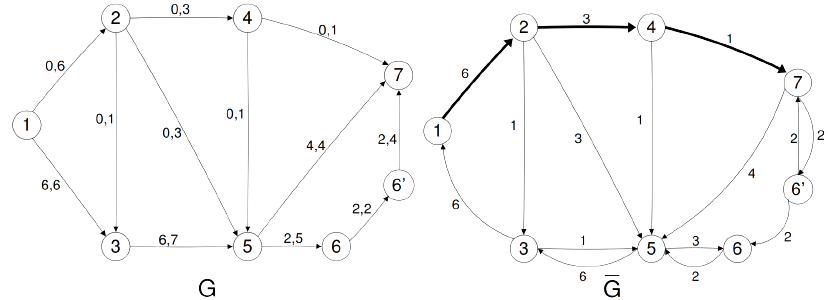
\includegraphics[width=0.9\linewidth]{images/max3.png}
        \end{figure}
        We send $\delta = 1$ additional units along the augmenting path \[\left\langle (1, 2),(2, 4),(4, 7) \right\rangle\]
        \begin{figure}[H]
            \centering
            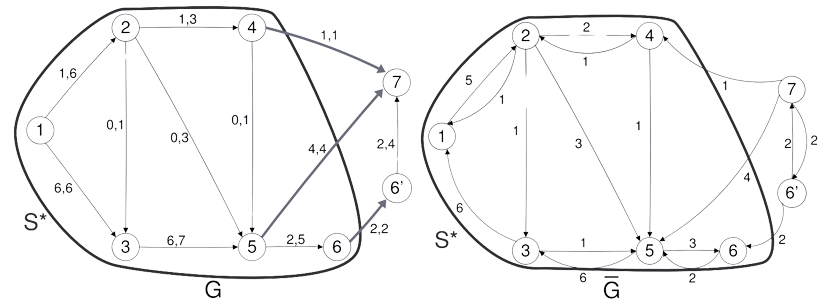
\includegraphics[width=0.9\linewidth]{images/max4.png}
        \end{figure}
        No other augmenting path exists. The minimum cut induced by $S^{*} = \{1, 2, 3, 4, 5, 6\}$ is highlighted in red. It has a total capacity $k(S^{*}) = \varphi = 7$.
  
    \newpage 

    \section{Indirect application of maximum flows}
        A software house has to handle 3 projects, $P_1$, $P_2$, $P_3$, over the next 4 months. The projects require 8, 10, and 12 man/months, respectively. $P_1$ can only 
        begin after month 1, and must be completed at latest by the end of month 3. $P_2$ and $P_3$ can begin from month 1, and must be completed by the end of month 4 and 
        2, respectively. Each month, 8 engineers are available. Due to the internal structure of the company, no more than 6 engineers can work, at the same time, on the 
        same project. Determine whether it is possible to complete the three projects within the time constraints and, if it is possible, find a feasible workforce plan. 
        Describe how this problem can be reduced to the problem of finding a maximum flow in an appropriate network.
    \subsection*{Solution}
        We build a network with nodes $m_1, m_2, m_3, m_4$ associated to the four months and nodes $P_1, P_2, P_3$ associated to the three projects.
        \begin{figure}[H]
            \centering
            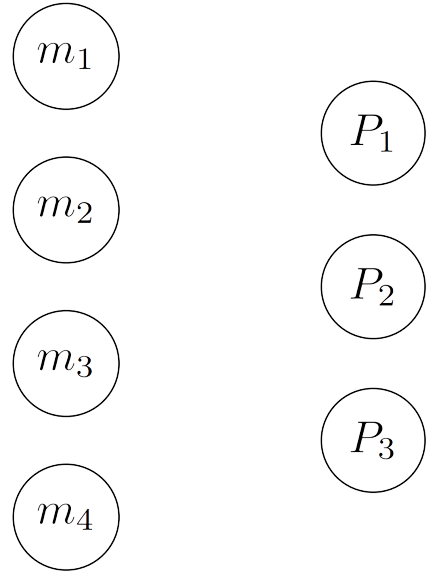
\includegraphics[width=0.2\linewidth]{images/indflow.png}
        \end{figure}
        For each pair of month-node mi and project-node $P_j$, the arc $(m_i, P_j)$ is included in the network if man/hours of month $i$ can be allocated to project $P_j$. 
        For instance, since project $P_1$ can only begin after month $1$ and must be completed within month $3$, there are only two arcs entering in $P_1$, namely $(m_2, P_1)$ 
        and $(m_3, P_1)$. Thus, we obtain the following bipartite oriented graph.
        \begin{figure}[H]
            \centering
            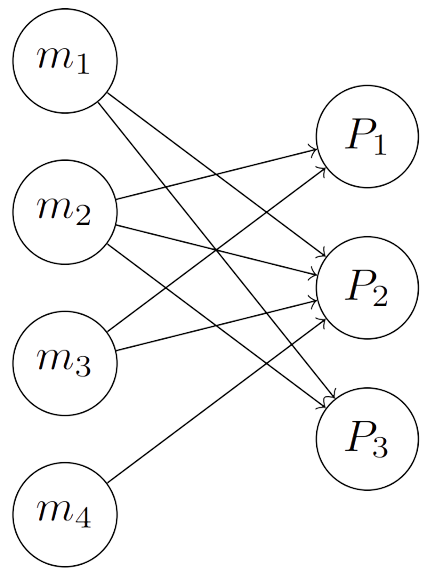
\includegraphics[width=0.2\linewidth]{images/inflow1.png}
        \end{figure}
        All arcs outgoing from $s$ have capacity 8, since there are 8 engineers available. All arcs connecting month-nodes to project-nodes have capacity 6, as no more than 6 engineers 
        can work on the same project at the same time. All arcs entering in $t$ have a capacity that is equivalent to the number of man/months needed to complete the corresponding 
        project $P_j$. All arcs outgoing from $s$ have capacity 8, since there are 8 engineers available. All arcs connecting month/nodes to project-nodes have capacity 6, as no more 
        than 6 engineers can work on the same project at the same time. All arcs entering in $t$ have a capacity that is equivalent to the number of man/months needed to complete the 
        corresponding project $P_j$.

        Since all capacities are integer, the maximum flow will be integer as well. To check whether all projects can be completed within the given time limits, it suffices to check 
        whether the network admits a feasible flow of value $8 + 10 + 12 = 30$.

        A feasible flow of maximum value $30$ can be found by applying Ford-Fulkerson algorithm. We can start from the feasible flow $\underline{x}_0 = 0$ of value $\varphi_0 = 0$ 
        and use the following augmenting paths:
        \begin{itemize}
            \item $\left\langle (s, m_3),(m_3, P_1),(P_1, t) \right\rangle$ with $\delta = 6$, yielding a feasible flow of value $\varphi_1 = 6$.
            \item $\left\langle (s, m_2),(m_2, P_1),(P_1, t) \right\rangle$ with $\delta = 2$, yielding a feasible flow of value $\varphi_2 = 8$.
            \item $\left\langle (s, m_1),(m_1, P_3),(P_3, t) \right\rangle$ with $\delta = 6$, yielding a feasible flow of value $\varphi_3 = 14$.
            \item $\left\langle (s, m_2),(m_2, P_3),(P_3, t) \right\rangle$ with $\delta = 6$, yielding a feasible flow of value $\varphi_4 = 20$.
            \item $\left\langle (s, m_4),(m_4, P_2),(P_2, t) \right\rangle$ with $\delta = 6$, yielding a feasible flow of value $\varphi_5 = 26$.
            \item $\left\langle (s, m_3),(m_1, P_2),(P_2, t) \right\rangle$ with $\delta = 2$, yielding a feasible flow of value $\varphi_6 = 28$.
            \item $\left\langle (s, m_3),(m_3, P_2),(P_2, t) \right\rangle$ with $\delta = 2$, yielding a feasible flow of value $\varphi_7 = 30$.
        \end{itemize}
        The resulting feasible flow $\underline{x}_7$ of value $\varphi_7 = 30$ is as follows.
        \begin{figure}[H]
            \centering
            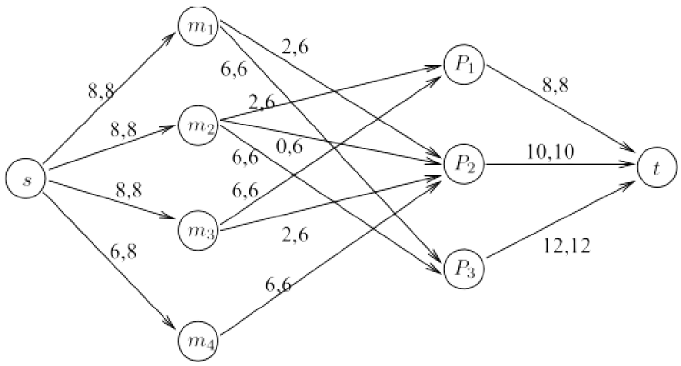
\includegraphics[width=0.5\linewidth]{images/inflow2.png}
        \end{figure}
        And the associated residual network $\overline{G}_7$ is the following. 
        \begin{figure}[H]
            \centering
            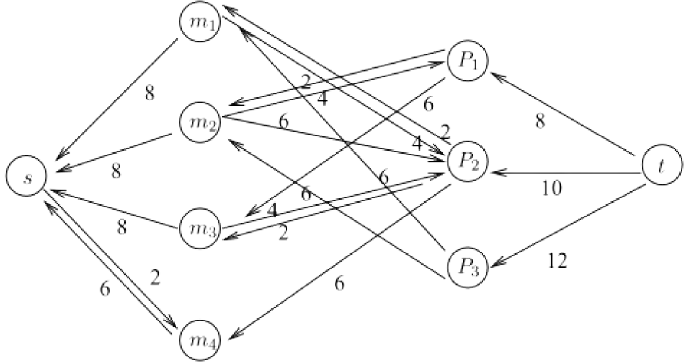
\includegraphics[width=0.5\linewidth]{images/inflow3.png}
        \end{figure}
        Note that in $\overline{G}_7$ only node $m_4$ can be reached from node $s$, hence $S^{*} = \{s, m_4\}$.
        
        Since the cut $\delta G(S^{*}) = \{(s, m_1),(s, m_2),(s, m_3),(m_4, P_2)\}$ has a total capacity of $k(S^{*}) =8 + 8 + 8 + 6 = 30$ which is equal to the value $\varphi_7 = 30$ of the feasible flow 
        $\underline{x}_7$, weak duality implies that the feasible flow $\underline{x}_7$ is of maximum value and the cut $\delta G(S^{*})$ is of minimum total capacity (among all the cuts separating the source 
        $s$ from the sink $t$).

\newpage

\chapter{Laboratory session I}
    \section{Linear programming modeling}
        A canteen has to plan the composition of the meals that it provides. A meal can be composed of the types of food indicated in the following table. 
        Costs, in Euro per hg, and availabilities, in hg, are also indicated.
        \begin{table}[H]
            \centering
            \begin{tabular}{|c|c|c|}
            \hline
            \textbf{Food} & \textbf{Cost} & \textbf{Availability} \\ \hline
            Bread         & 0.1           & 4                     \\
            Milk          & 0.5           & 3                     \\
            Eggs          & 0.12          & 1                     \\
            Meat          & 0.9           & 2                     \\
            Cake          & 1.3           & 2                     \\ \hline
            \end{tabular}
        \end{table}
        A meal must contain at least the following amount of each nutrient: 
        \begin{table}[H]
            \centering
            \begin{tabular}{|c|c|}
            \hline
            Nutrient & Minimal quantity \\ \hline
            Calories & 600 cal          \\
            Proteins & 50 g             \\
            Calcium  & 0.7 g            \\ \hline
            \end{tabular}
        \end{table}
        Each hg of each type of food contains to following amount of nutrients: 
        \begin{table}[H]
            \centering
            \begin{tabular}{|cccc|}
            \hline
            \textbf{Food}               & \textbf{Calories}            & \textbf{Proteins}         & \textbf{Calcium} \\ \hline
            \multicolumn{1}{|c|}{Bread} & \multicolumn{1}{c|}{30 cal}  & \multicolumn{1}{c|}{15 g} & 0.02 g           \\
            \multicolumn{1}{|c|}{Milk}  & \multicolumn{1}{c|}{50 cal}  & \multicolumn{1}{c|}{15 g} & 0.15 g           \\
            \multicolumn{1}{|c|}{Eggs}  & \multicolumn{1}{c|}{150 cal} & \multicolumn{1}{c|}{30 g} & 0.05 g           \\
            \multicolumn{1}{|c|}{Meat}  & \multicolumn{1}{c|}{180 cal} & \multicolumn{1}{c|}{90 g} & 0.08 g           \\
            \multicolumn{1}{|c|}{Cake}  & \multicolumn{1}{c|}{400 cal} & \multicolumn{1}{c|}{70 g} & 0.01 g           \\ \hline
            \end{tabular}
        \end{table}
        Give a linear programming formulation for the problem of finding a meal of minimum total cost which satisfies the minimum nutrient requirements.
    \subsection*{Solution}
        \begin{lstlisting}[style=Python]
# Import the package mip
!pip install mip
import mip
# Food
I = {'Bread', 'Milk', 'Eggs', 'Meat', 'Cake'}
# Nutrients
J = {'Calories', 'Proteins', 'Calcium'}
# Cost in Euro per hg of food
c = {'Bread':0.1, 'Milk':0.5, 'Eggs':0.12, 'Meat':0.9, 'Cake':1.3}
# Availability per hg of food
q = {'Bread':4, 'Milk':3, 'Eggs':1, 'Meat':2, 'Cake':2}
# minum nutrients 
b = {'Calories':600, 'Proteins':50, 'Calcium':0.7}
# Nutrients per hf of food
a = {   ('Bread','Calories'):30,
        ('Milk','Calories'):50,
        ('Eggs','Calories'):150,
        ('Meat','Calories'):180,
        ('Cake','Calories'):400,
        ('Bread','Proteins'):5,
        ('Milk','Proteins'):15,
        ('Eggs','Proteins'):30,
        ('Meat','Proteins'):90,
        ('Cake','Proteins'):70,
        ('Bread','Calcium'):0.02,
        ('Milk','Calcium'):0.15,
        ('Eggs','Calcium'):0.05,
        ('Meat','Calcium'):0.08,
        ('Cake','Calcium'):0.01}
# Define a empty model
model = mip.Model()
# Define variables
x = [model.add_var(name = i,lb=0) for i in I]
# Define the objective function
model.objective = mip.minimize(mip.xsum())
# Availability constraint
for i,food in enumerate(I):
model.add_constr()
# Minum nutrients constraint
for j in J:
model.add_constr(mip.xsum()>=)
# Optimizing command
model.optimize()
# Optimal objective function value
model.objective.x
# Printing the variables values
for i in model.vars:
print(i.name)
print(i.x)
        \end{lstlisting}
    
\end{document}